\chapter{Porte logiche in tecnologia c-MOS}
	
	I principali componenti attuali utilizzati nei dispositivi digitali sono realizzati mediante l'implementazione su chip di transistor opportunamente connessi. Come visto i mosfet sono degli oggetti che sono intrinsecamente analogici, tuttavia il loro principio di funzionamento li rende altamente adatti a realizzare funzioni digitali.
	
	A livello digitale infatti i transistor possono essere considerati come degli interruttori che permettono o negano il passaggio di corrente tra i propri terminali. Considerando infatti la caratteristica statica dell'n-mos (figura \ref{fig:intro:nmos-carattstatica}, pagina \pageref{fig:intro:nmos-carattstatica}) è possibile osservare che se si pone una tensione di gate $V_g$ nulla (più in generale inferiore della tensione di soglia $\Vtn$) il dispositivo non permette il passaggio di corrente ai suoi capi (indipendentemente dalla tensione differenziale $V_{ds}$ applicata); usciti dalla fascia di interdizione è possibile osservare invece che, in funzione della tensione $\Vgs$, è possibile avere un passaggio di corrente attraverso i terminali del mosfet.\\
	Dualmente si dimostra che se la tensione $V_g$ applicata al gate di un transitor p-mos è elevata (tale per cui la differenza $|V_{gs}|$ sia minore della tensione di soglia $|V_{tp}|$) allora il componente risulta interdetto e non permette il passaggio di corrente.
	
	Questa peculiarità nel funzionamento duale dei componenti è particolarmente utile nelle implementazioni digitali dove in generale si considerano i segnali di tensione (intrinsecamente analogici) come dei segnali binari di valore basso (0) associato alla tensione di massa e valore alto (1) associato alla tensione di alimentazione $V_{dd}$.
	
	Lo scopo di questo capitolo è dunque quello di osservare e rappresentare le porte logiche che compongono ogni circuito combinatorio di un dispositivo tecnologico.

\section{Not gate}
	
	La porta logica più semplice da realizzare, composta da solamente due transistori, è il \textit{gate not}, ossia l'invertitore logico che realizza la seguente tabella di verità:
	\begin{center}
	\begin{tabular}{c | c}
			input & output \\ \hline
			0 & 1 \\ 1 & 0
	\end{tabular}
	\end{center}
	
	L'implementazione circuitale di questa porta è mostrata in figura \ref{fig:not:schematico} ed è realizzata ponendo in serie un p-mos con un n-mos: l'ingresso $V_{in}$ del segnale digitale viene applicato ad entrambi i gate dei transistor, mentre il segnale in uscita $V_{out}$ viene rilevato nel collegamento tra i due drain dei mosfet.
	
	\begin{figure}[bht]
		\centering
		\begin{subfigure}{0.48\linewidth}
			\centering
			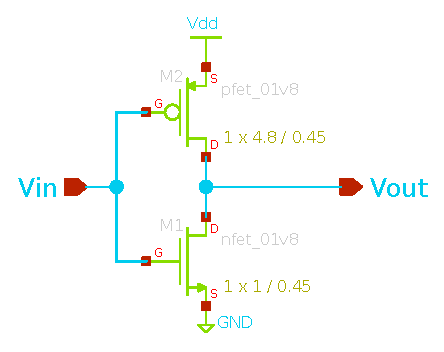
\includegraphics[width=5cm]{Immagini/not-gate.eps} \caption{}			
		\end{subfigure}
		\begin{subfigure}{0.48\linewidth}
			\centering
			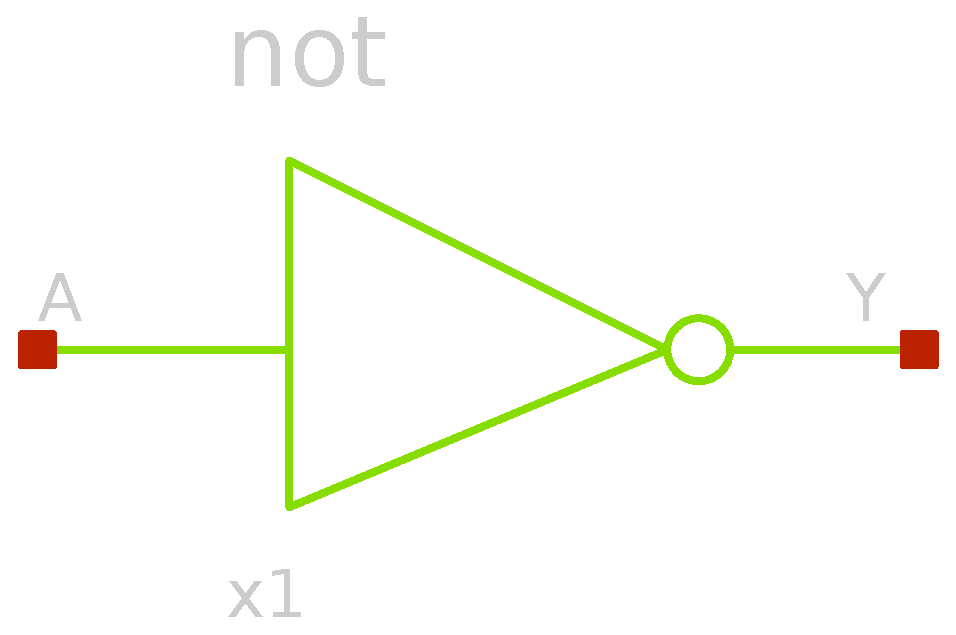
\includegraphics[width=2.5cm]{Immagini/not-gate-simple.eps} \caption{}			
		\end{subfigure}
		\caption{implementazione di un invertitore logico in tecnologia c-mos (a) e relativa rappresentazione simbolica per circuiti logici (b).} 
		\label{fig:not:schematico}
	\end{figure}
	
	Per comprendere il funzionamento del sistema è sufficiente considerare la prima legge di Kirchhoff bilanciando la corrente al nodo rispetto alla quale si rileva il segnale in uscita $\Vout$ che si traduce nell'eguagliare le correnti generate dai due transistor:
	\[ I_n = I_p \]
	
	A questo punto è possibile procedere con l'analisi del circuito per casi:
	\begin{itemize}
		\item nel caso in cui la tensione in ingresso sia bassa ($V_{in} = 0$) allora l'n-mos risulterebbe essere interdetto ($I_n = 0$), mentre il p-mos è posto in regime di saturazione. L'unica condizione che permette al p-mos di non far scorrere corrente attraverso i suoi terminali è quella per cui la tensione differenziale $V_{ds}$ è nulla: questo porta ad affermare che
		\[ V_d = V_s \qquad \Rightarrow \qquad V_{out} = V_{dd} \]
		
		\item analogamente nel caso in cui l'ingresso si trovi ad una tensione in ingresso alta ($V_{in} = V_{dd}$), il p-mos risulterà interdetto, non permettendo il passaggio di alcuna corrente. Condizione necessaria affinché anche l'n-mos annulli la corrente attraverso i suoi terminali è che la tensione differenziale $V_{ds}$ sia nulla, e dunque
		\[ V_{out} = 0 \]
	\end{itemize} 
	
	In figura \ref{fig:not:carattstatica} è possibile invece osservare la caratteristica statica del dispositivo ottenuta mediante una simulazione.
	
	\begin{figure}[H]
		\centering
		% GNUPLOT: LaTeX picture with Postscript
\begingroup
  \makeatletter
  \providecommand\color[2][]{%
    \GenericError{(gnuplot) \space\space\space\@spaces}{%
      Package color not loaded in conjunction with
      terminal option `colourtext'%
    }{See the gnuplot documentation for explanation.%
    }{Either use 'blacktext' in gnuplot or load the package
      color.sty in LaTeX.}%
    \renewcommand\color[2][]{}%
  }%
  \providecommand\includegraphics[2][]{%
    \GenericError{(gnuplot) \space\space\space\@spaces}{%
      Package graphicx or graphics not loaded%
    }{See the gnuplot documentation for explanation.%
    }{The gnuplot epslatex terminal needs graphicx.sty or graphics.sty.}%
    \renewcommand\includegraphics[2][]{}%
  }%
  \providecommand\rotatebox[2]{#2}%
  \@ifundefined{ifGPcolor}{%
    \newif\ifGPcolor
    \GPcolorfalse
  }{}%
  \@ifundefined{ifGPblacktext}{%
    \newif\ifGPblacktext
    \GPblacktexttrue
  }{}%
  % define a \g@addto@macro without @ in the name:
  \let\gplgaddtomacro\g@addto@macro
  % define empty templates for all commands taking text:
  \gdef\gplbacktext{}%
  \gdef\gplfronttext{}%
  \makeatother
  \ifGPblacktext
    % no textcolor at all
    \def\colorrgb#1{}%
    \def\colorgray#1{}%
  \else
    % gray or color?
    \ifGPcolor
      \def\colorrgb#1{\color[rgb]{#1}}%
      \def\colorgray#1{\color[gray]{#1}}%
      \expandafter\def\csname LTw\endcsname{\color{white}}%
      \expandafter\def\csname LTb\endcsname{\color{black}}%
      \expandafter\def\csname LTa\endcsname{\color{black}}%
      \expandafter\def\csname LT0\endcsname{\color[rgb]{1,0,0}}%
      \expandafter\def\csname LT1\endcsname{\color[rgb]{0,1,0}}%
      \expandafter\def\csname LT2\endcsname{\color[rgb]{0,0,1}}%
      \expandafter\def\csname LT3\endcsname{\color[rgb]{1,0,1}}%
      \expandafter\def\csname LT4\endcsname{\color[rgb]{0,1,1}}%
      \expandafter\def\csname LT5\endcsname{\color[rgb]{1,1,0}}%
      \expandafter\def\csname LT6\endcsname{\color[rgb]{0,0,0}}%
      \expandafter\def\csname LT7\endcsname{\color[rgb]{1,0.3,0}}%
      \expandafter\def\csname LT8\endcsname{\color[rgb]{0.5,0.5,0.5}}%
    \else
      % gray
      \def\colorrgb#1{\color{black}}%
      \def\colorgray#1{\color[gray]{#1}}%
      \expandafter\def\csname LTw\endcsname{\color{white}}%
      \expandafter\def\csname LTb\endcsname{\color{black}}%
      \expandafter\def\csname LTa\endcsname{\color{black}}%
      \expandafter\def\csname LT0\endcsname{\color{black}}%
      \expandafter\def\csname LT1\endcsname{\color{black}}%
      \expandafter\def\csname LT2\endcsname{\color{black}}%
      \expandafter\def\csname LT3\endcsname{\color{black}}%
      \expandafter\def\csname LT4\endcsname{\color{black}}%
      \expandafter\def\csname LT5\endcsname{\color{black}}%
      \expandafter\def\csname LT6\endcsname{\color{black}}%
      \expandafter\def\csname LT7\endcsname{\color{black}}%
      \expandafter\def\csname LT8\endcsname{\color{black}}%
    \fi
  \fi
    \setlength{\unitlength}{0.0500bp}%
    \ifx\gptboxheight\undefined%
      \newlength{\gptboxheight}%
      \newlength{\gptboxwidth}%
      \newsavebox{\gptboxtext}%
    \fi%
    \setlength{\fboxrule}{0.5pt}%
    \setlength{\fboxsep}{1pt}%
\begin{picture}(4250.00,2154.00)%
    \gplgaddtomacro\gplbacktext{%
      \csname LTb\endcsname%%
      \put(814,704){\makebox(0,0)[r]{\strut{}$0$}}%
      \csname LTb\endcsname%%
      \put(814,909){\makebox(0,0)[r]{\strut{}$0.3$}}%
      \csname LTb\endcsname%%
      \put(814,1114){\makebox(0,0)[r]{\strut{}$0.6$}}%
      \csname LTb\endcsname%%
      \put(814,1319){\makebox(0,0)[r]{\strut{}$0.9$}}%
      \csname LTb\endcsname%%
      \put(814,1523){\makebox(0,0)[r]{\strut{}$1.2$}}%
      \csname LTb\endcsname%%
      \put(814,1728){\makebox(0,0)[r]{\strut{}$1.5$}}%
      \csname LTb\endcsname%%
      \put(814,1933){\makebox(0,0)[r]{\strut{}$1.8$}}%
      \csname LTb\endcsname%%
      \put(946,484){\makebox(0,0){\strut{}$0$}}%
      \csname LTb\endcsname%%
      \put(1431,484){\makebox(0,0){\strut{}$0.3$}}%
      \csname LTb\endcsname%%
      \put(1915,484){\makebox(0,0){\strut{}$0.6$}}%
      \csname LTb\endcsname%%
      \put(2400,484){\makebox(0,0){\strut{}$0.9$}}%
      \csname LTb\endcsname%%
      \put(2884,484){\makebox(0,0){\strut{}$1.2$}}%
      \csname LTb\endcsname%%
      \put(3369,484){\makebox(0,0){\strut{}$1.5$}}%
      \csname LTb\endcsname%%
      \put(3853,484){\makebox(0,0){\strut{}$1.8$}}%
    }%
    \gplgaddtomacro\gplfronttext{%
      \csname LTb\endcsname%%
      \put(209,1318){\rotatebox{-270}{\makebox(0,0){\strut{}$V_{out}$ $[V]$}}}%
      \put(2399,154){\makebox(0,0){\strut{}$V_{in}$ $[V]$}}%
      \csname LTb\endcsname%%
      \put(2399,6582){\makebox(0,0){\strut{}}}%
    }%
    \gplbacktext
    \put(0,0){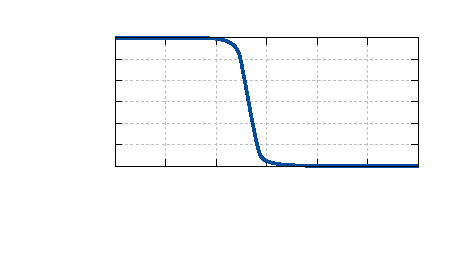
\includegraphics[width={212.50bp},height={107.70bp}]{Immagini/not_caratt}}%
    \gplfronttext
  \end{picture}%
\endgroup


		\caption{funzione di trasferimento statica dell'invertitore logico di figura \ref{fig:not:schematico}.}
		\label{fig:not:carattstatica}
	\end{figure}

	L'implementazione delle porte logiche in tecnologia c-mos è caratterizzata da una forte immunità al rumore. Definendo infatti con $V_{ilmax}$ la massima tensione a cui è associato una corrispondenza con il segnale basso (ossia ogni tensione $V<V_{ilmax}$ è considerato un 0 binario) e con $V_{ihmin}$ la minima tensione in ingresso riconosciuta come segnale alto, dall'analisi della caratteristica di trasferimento (figura \ref{fig:not:carattstatica}) si osserva che i valori ad esso associati sono circa $V_{ilmax} =0.6V$ e $V_{ihmin} = 0.9V$ rispetto ad una tensione di alimentazione $V_{dd} = 1.8V$. Questo significa che il segnale in uscita da una porta logica a valle può acquisire fino a $0.6V$ di rumore senza inficiare sul corretto funzionamento del circuito in quanto il segnale verrebbe ricevuto e considerato correttamente.
	
	\subsection*{Caratteristiche dinamiche}
		
		Nota la caratteristica statica del circuito logico, di rilevante interesse pratico è l'analisi dinamica dello stesso, in quanto permetterà di stabilire a regime quale sarà la massima frequenza di commutazione della porta logica.
		
		\begin{figure}[bht]
			\centering
			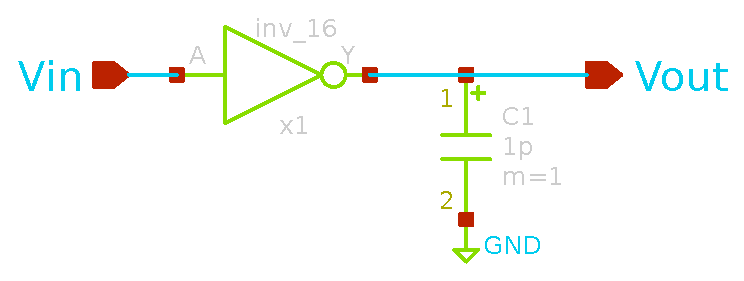
\includegraphics[width=5cm]{Immagini/not-gate-carico}
			\caption{schema circuitale di riferimento per l'analisi della risposta dinamica di un invertitore logico che deve pilotare un circuito a valle modellato da una capacità di $0.75pF$.}
			\label{fig:not:dinamica-schema}
		\end{figure}
		
		A tale fine è necessario considerare un'invertitore, come in figura \ref{fig:not:dinamica-schema}, che pilota un circuito a valle che può essere modellato, come indicato nella documentazione di skywater \cite{specprimitivecells}, mediante una capacità di carico $C_{load}$ collegata all'uscita di valore $0.75pF$.
	
		\begin{figure}[bht]
			\centering
			% GNUPLOT: LaTeX picture with Postscript
\begingroup
  \makeatletter
  \providecommand\color[2][]{%
    \GenericError{(gnuplot) \space\space\space\@spaces}{%
      Package color not loaded in conjunction with
      terminal option `colourtext'%
    }{See the gnuplot documentation for explanation.%
    }{Either use 'blacktext' in gnuplot or load the package
      color.sty in LaTeX.}%
    \renewcommand\color[2][]{}%
  }%
  \providecommand\includegraphics[2][]{%
    \GenericError{(gnuplot) \space\space\space\@spaces}{%
      Package graphicx or graphics not loaded%
    }{See the gnuplot documentation for explanation.%
    }{The gnuplot epslatex terminal needs graphicx.sty or graphics.sty.}%
    \renewcommand\includegraphics[2][]{}%
  }%
  \providecommand\rotatebox[2]{#2}%
  \@ifundefined{ifGPcolor}{%
    \newif\ifGPcolor
    \GPcolorfalse
  }{}%
  \@ifundefined{ifGPblacktext}{%
    \newif\ifGPblacktext
    \GPblacktexttrue
  }{}%
  % define a \g@addto@macro without @ in the name:
  \let\gplgaddtomacro\g@addto@macro
  % define empty templates for all commands taking text:
  \gdef\gplbacktext{}%
  \gdef\gplfronttext{}%
  \makeatother
  \ifGPblacktext
    % no textcolor at all
    \def\colorrgb#1{}%
    \def\colorgray#1{}%
  \else
    % gray or color?
    \ifGPcolor
      \def\colorrgb#1{\color[rgb]{#1}}%
      \def\colorgray#1{\color[gray]{#1}}%
      \expandafter\def\csname LTw\endcsname{\color{white}}%
      \expandafter\def\csname LTb\endcsname{\color{black}}%
      \expandafter\def\csname LTa\endcsname{\color{black}}%
      \expandafter\def\csname LT0\endcsname{\color[rgb]{1,0,0}}%
      \expandafter\def\csname LT1\endcsname{\color[rgb]{0,1,0}}%
      \expandafter\def\csname LT2\endcsname{\color[rgb]{0,0,1}}%
      \expandafter\def\csname LT3\endcsname{\color[rgb]{1,0,1}}%
      \expandafter\def\csname LT4\endcsname{\color[rgb]{0,1,1}}%
      \expandafter\def\csname LT5\endcsname{\color[rgb]{1,1,0}}%
      \expandafter\def\csname LT6\endcsname{\color[rgb]{0,0,0}}%
      \expandafter\def\csname LT7\endcsname{\color[rgb]{1,0.3,0}}%
      \expandafter\def\csname LT8\endcsname{\color[rgb]{0.5,0.5,0.5}}%
    \else
      % gray
      \def\colorrgb#1{\color{black}}%
      \def\colorgray#1{\color[gray]{#1}}%
      \expandafter\def\csname LTw\endcsname{\color{white}}%
      \expandafter\def\csname LTb\endcsname{\color{black}}%
      \expandafter\def\csname LTa\endcsname{\color{black}}%
      \expandafter\def\csname LT0\endcsname{\color{black}}%
      \expandafter\def\csname LT1\endcsname{\color{black}}%
      \expandafter\def\csname LT2\endcsname{\color{black}}%
      \expandafter\def\csname LT3\endcsname{\color{black}}%
      \expandafter\def\csname LT4\endcsname{\color{black}}%
      \expandafter\def\csname LT5\endcsname{\color{black}}%
      \expandafter\def\csname LT6\endcsname{\color{black}}%
      \expandafter\def\csname LT7\endcsname{\color{black}}%
      \expandafter\def\csname LT8\endcsname{\color{black}}%
    \fi
  \fi
    \setlength{\unitlength}{0.0500bp}%
    \ifx\gptboxheight\undefined%
      \newlength{\gptboxheight}%
      \newlength{\gptboxwidth}%
      \newsavebox{\gptboxtext}%
    \fi%
    \setlength{\fboxrule}{0.5pt}%
    \setlength{\fboxsep}{1pt}%
\begin{picture}(5668.00,2550.00)%
    \gplgaddtomacro\gplbacktext{%
      \csname LTb\endcsname%%
      \put(434,1550){\makebox(0,0)[r]{\strut{}$0$}}%
      \csname LTb\endcsname%%
      \put(434,1988){\makebox(0,0)[r]{\strut{}$0.9$}}%
      \csname LTb\endcsname%%
      \put(434,2426){\makebox(0,0)[r]{\strut{}$1.8$}}%
      \csname LTb\endcsname%%
      \put(566,1233){\makebox(0,0){\strut{}}}%
      \csname LTb\endcsname%%
      \put(1529,1233){\makebox(0,0){\strut{}}}%
      \csname LTb\endcsname%%
      \put(2493,1233){\makebox(0,0){\strut{}}}%
      \csname LTb\endcsname%%
      \put(3456,1233){\makebox(0,0){\strut{}}}%
      \csname LTb\endcsname%%
      \put(4420,1233){\makebox(0,0){\strut{}}}%
      \csname LTb\endcsname%%
      \put(5383,1233){\makebox(0,0){\strut{}}}%
    }%
    \gplgaddtomacro\gplfronttext{%
      \csname LTb\endcsname%%
      \put(-171,1988){\rotatebox{-270}{\makebox(0,0){\strut{}$V_{out}$}}}%
      \put(2974,1167){\makebox(0,0){\strut{}}}%
    }%
    \gplgaddtomacro\gplbacktext{%
      \csname LTb\endcsname%%
      \put(434,479){\makebox(0,0)[r]{\strut{}$0$}}%
      \csname LTb\endcsname%%
      \put(434,917){\makebox(0,0)[r]{\strut{}$0.9$}}%
      \csname LTb\endcsname%%
      \put(434,1355){\makebox(0,0)[r]{\strut{}$1.8$}}%
      \csname LTb\endcsname%%
      \put(566,162){\makebox(0,0){\strut{}0}}%
      \csname LTb\endcsname%%
      \put(1529,162){\makebox(0,0){\strut{}10}}%
      \csname LTb\endcsname%%
      \put(2493,162){\makebox(0,0){\strut{}20}}%
      \csname LTb\endcsname%%
      \put(3456,162){\makebox(0,0){\strut{}30}}%
      \csname LTb\endcsname%%
      \put(4420,162){\makebox(0,0){\strut{}40}}%
      \csname LTb\endcsname%%
      \put(5383,162){\makebox(0,0){\strut{}50}}%
    }%
    \gplgaddtomacro\gplfronttext{%
      \csname LTb\endcsname%%
      \put(-171,917){\rotatebox{-270}{\makebox(0,0){\strut{}$V_{in}$}}}%
      \put(2974,-168){\makebox(0,0){\strut{}tempo $[ns]$}}%
    }%
    \gplbacktext
    \put(0,0){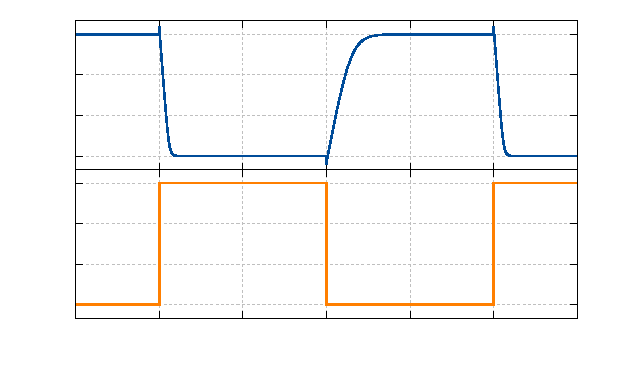
\includegraphics[width={283.40bp},height={127.50bp}]{Immagini/not-dinamica}}%
    \gplfronttext
  \end{picture}%
\endgroup


			\vspace{2mm}
			\caption{risposta dell'invertitore logico (in figura \ref{fig:not:dinamica-schema}) ad un'onda quadra in ingresso di periodo $30ns$ e duty cycle del $50\%$.  Le tensioni sono espresse in volt.}
			\label{fig:not:dinamica}
		\end{figure}
		
		In figura \ref{fig:not:dinamica} è possibile leggere la risposta dell'invertitore ad un'onda quadra in ingresso. Data la simmetricità di comportamento scelta grazie ai rapporti $W/L$ diversi dei transistor p-mos ed n-mos è possibile osservare che i transistori di salita e discesa sono molto simili tra loro.
		
		Rispetto al valore della capacità scelto di $0.75pF$ (considerato rappresentativo di un generico circuito a valle) è possibile valutare i ritardi di propagazione dei segnali, ossia i tempi che intercorrono tra le commutazioni dell'ingresso e la rispettiva variazione d'uscita. \\		
		Tali parametri possono essere valutati singolarmente sia per una variazione dell'ingresso da alto a basso $\tau_{hl}$, ma anche per lo stesso che passa da basso a alto $\tau_{lh}$ (in questo caso i tempi sono calcolati al $95\%$ dell'escursione di tensione):
		\[ \tau_{lh} = 7.21ns \qquad \tau_{hl} = 7.14ns  \] 



\section{Nor gate}
	La porta logica \textit{nor}, coincidente con la negazione del gate \textit{or}, è un gate che, come il \textit{nand}, costituisce un \textit{operatore universale}, ossia in grado di realizzare tramite delle opportune interconnessioni tutte le funzioni logiche digitali. Tale porta a due (o più ingressi) rispetta la seguente tabella di verità:
	\begin{center}
		\begin{tabular}{c c | c}
			$V_{in,1}$ & $V_{in,2}$ & $V_{out}$ \\ \hline
			0 & 0 & 1 \\
			0 & 1 & 0 \\
			1 & 0 & 0 \\
			1 & 1 & 0 \\
		\end{tabular}
	\end{center}
	Si osserva dunque che tale porta logica determina un'uscita alta solamente se tutti i suoi ingressi sono bassi, mentre in tutti gli altri casi l'uscita è bassa.
	
	\begin{figure}[bht]
		\centering
		\begin{subfigure}{0.48\linewidth}
			\centering
			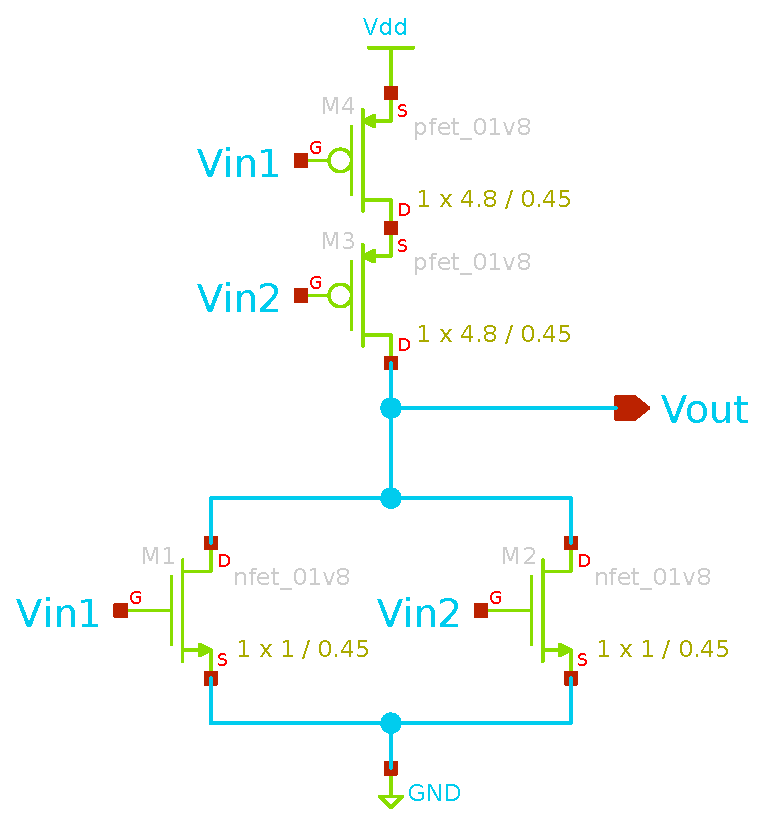
\includegraphics[width=5cm]{Immagini/nor-gate.eps} \caption{}			
		\end{subfigure}
		\begin{subfigure}{0.48\linewidth}
			\centering
			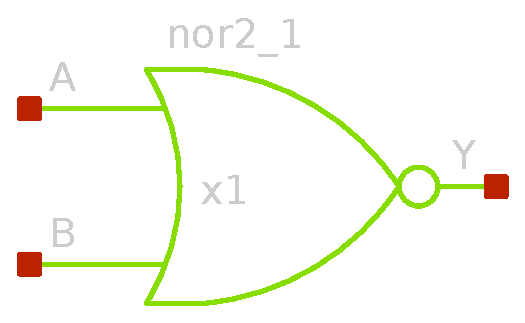
\includegraphics[width=2.5cm]{Immagini/nor-gate-simple.eps} \caption{}			
		\end{subfigure}
		\caption{implementazione della porta logica nor in tecnologia c-mos (a) e la relativa rappresentazione schematica (b).}
		\label{fig:nor:schematico}
	\end{figure}

	In figura \ref{fig:nor:schematico} è dunque possibile osservare un'implementazione della porta logica nor in tecnologia c-mos.\\
	Tale circuito può essere descritto analizzando le possibili combinazioni di ingresso presenti nella tabella di verità:
	\begin{itemize}
		\item nel caso in cui entrambi gli ingressi si trovino ad un valore basso (prima riga della tabella di verità), allora risulterebbero interdetti i transistor a substrato n, mentre la rete di pull-up composta dai due p-mos in serie risulterebbe essere attiva. L'unico modo per garantire corrente nulla in uscita dal circuito è quello di avere tensione differenziale $V_{ds}$ dei p-mos nulla, ossia nel caso in cui $V_{out} = V_{dd}$, verificando la tabella di verità;
		
		\item in tutti gli altri casi in cui almeno un segnale si trova in uno stato di tensione alto si osserva che la rete di pull-up sarà sicuramente interdetta (il p-mos associato all'ingresso alto non permetterebbe infatti passaggio di corrente), e dunque la tensione in uscita sarà determinata dalla rete di pull-down degli n-mos che risulteranno attivi. Sempre per imposizione della condizione di corrente nulla al nodo d'uscita si ottiene che la tensione differenziale $V_{ds}$ degli n-mos deve essere nulla e dunque $V_{out} = 0$.
	\end{itemize}
	
	Tale comportamento può essere verificato mediante una simulazione del transitorio (il cui risultato è mostrato in figura \ref{fig:nor:dinamica}), imponendo come ingressi delle onde quadre di periodo multiplo per analizzare le risposte del circuito alle varie combinazioni di ingressi e determinare così le principali caratteristiche dinamiche.
	
	\begin{figure}[bht]
		\centering
		% GNUPLOT: LaTeX picture with Postscript
\begingroup
  \makeatletter
  \providecommand\color[2][]{%
    \GenericError{(gnuplot) \space\space\space\@spaces}{%
      Package color not loaded in conjunction with
      terminal option `colourtext'%
    }{See the gnuplot documentation for explanation.%
    }{Either use 'blacktext' in gnuplot or load the package
      color.sty in LaTeX.}%
    \renewcommand\color[2][]{}%
  }%
  \providecommand\includegraphics[2][]{%
    \GenericError{(gnuplot) \space\space\space\@spaces}{%
      Package graphicx or graphics not loaded%
    }{See the gnuplot documentation for explanation.%
    }{The gnuplot epslatex terminal needs graphicx.sty or graphics.sty.}%
    \renewcommand\includegraphics[2][]{}%
  }%
  \providecommand\rotatebox[2]{#2}%
  \@ifundefined{ifGPcolor}{%
    \newif\ifGPcolor
    \GPcolorfalse
  }{}%
  \@ifundefined{ifGPblacktext}{%
    \newif\ifGPblacktext
    \GPblacktexttrue
  }{}%
  % define a \g@addto@macro without @ in the name:
  \let\gplgaddtomacro\g@addto@macro
  % define empty templates for all commands taking text:
  \gdef\gplbacktext{}%
  \gdef\gplfronttext{}%
  \makeatother
  \ifGPblacktext
    % no textcolor at all
    \def\colorrgb#1{}%
    \def\colorgray#1{}%
  \else
    % gray or color?
    \ifGPcolor
      \def\colorrgb#1{\color[rgb]{#1}}%
      \def\colorgray#1{\color[gray]{#1}}%
      \expandafter\def\csname LTw\endcsname{\color{white}}%
      \expandafter\def\csname LTb\endcsname{\color{black}}%
      \expandafter\def\csname LTa\endcsname{\color{black}}%
      \expandafter\def\csname LT0\endcsname{\color[rgb]{1,0,0}}%
      \expandafter\def\csname LT1\endcsname{\color[rgb]{0,1,0}}%
      \expandafter\def\csname LT2\endcsname{\color[rgb]{0,0,1}}%
      \expandafter\def\csname LT3\endcsname{\color[rgb]{1,0,1}}%
      \expandafter\def\csname LT4\endcsname{\color[rgb]{0,1,1}}%
      \expandafter\def\csname LT5\endcsname{\color[rgb]{1,1,0}}%
      \expandafter\def\csname LT6\endcsname{\color[rgb]{0,0,0}}%
      \expandafter\def\csname LT7\endcsname{\color[rgb]{1,0.3,0}}%
      \expandafter\def\csname LT8\endcsname{\color[rgb]{0.5,0.5,0.5}}%
    \else
      % gray
      \def\colorrgb#1{\color{black}}%
      \def\colorgray#1{\color[gray]{#1}}%
      \expandafter\def\csname LTw\endcsname{\color{white}}%
      \expandafter\def\csname LTb\endcsname{\color{black}}%
      \expandafter\def\csname LTa\endcsname{\color{black}}%
      \expandafter\def\csname LT0\endcsname{\color{black}}%
      \expandafter\def\csname LT1\endcsname{\color{black}}%
      \expandafter\def\csname LT2\endcsname{\color{black}}%
      \expandafter\def\csname LT3\endcsname{\color{black}}%
      \expandafter\def\csname LT4\endcsname{\color{black}}%
      \expandafter\def\csname LT5\endcsname{\color{black}}%
      \expandafter\def\csname LT6\endcsname{\color{black}}%
      \expandafter\def\csname LT7\endcsname{\color{black}}%
      \expandafter\def\csname LT8\endcsname{\color{black}}%
    \fi
  \fi
    \setlength{\unitlength}{0.0500bp}%
    \ifx\gptboxheight\undefined%
      \newlength{\gptboxheight}%
      \newlength{\gptboxwidth}%
      \newsavebox{\gptboxtext}%
    \fi%
    \setlength{\fboxrule}{0.5pt}%
    \setlength{\fboxsep}{1pt}%
\begin{picture}(5668.00,3118.00)%
    \gplgaddtomacro\gplbacktext{%
      \csname LTb\endcsname%%
      \put(434,2292){\makebox(0,0)[r]{\strut{}$0$}}%
      \csname LTb\endcsname%%
      \put(434,2649){\makebox(0,0)[r]{\strut{}$0.9$}}%
      \csname LTb\endcsname%%
      \put(434,3006){\makebox(0,0)[r]{\strut{}$1.8$}}%
      \csname LTb\endcsname%%
      \put(566,1993){\makebox(0,0){\strut{}}}%
      \csname LTb\endcsname%%
      \put(1369,1993){\makebox(0,0){\strut{}}}%
      \csname LTb\endcsname%%
      \put(2172,1993){\makebox(0,0){\strut{}}}%
      \csname LTb\endcsname%%
      \put(2975,1993){\makebox(0,0){\strut{}}}%
      \csname LTb\endcsname%%
      \put(3777,1993){\makebox(0,0){\strut{}}}%
      \csname LTb\endcsname%%
      \put(4580,1993){\makebox(0,0){\strut{}}}%
      \csname LTb\endcsname%%
      \put(5383,1993){\makebox(0,0){\strut{}}}%
    }%
    \gplgaddtomacro\gplfronttext{%
      \csname LTb\endcsname%%
      \put(-171,2649){\rotatebox{-270}{\makebox(0,0){\strut{}$V_{out}$}}}%
      \put(2974,1927){\makebox(0,0){\strut{}}}%
    }%
    \gplgaddtomacro\gplbacktext{%
      \csname LTb\endcsname%%
      \put(434,1419){\makebox(0,0)[r]{\strut{}$0$}}%
      \csname LTb\endcsname%%
      \put(434,1777){\makebox(0,0)[r]{\strut{}$0.9$}}%
      \csname LTb\endcsname%%
      \put(434,2134){\makebox(0,0)[r]{\strut{}$1.8$}}%
      \csname LTb\endcsname%%
      \put(566,1120){\makebox(0,0){\strut{}}}%
      \csname LTb\endcsname%%
      \put(1369,1120){\makebox(0,0){\strut{}}}%
      \csname LTb\endcsname%%
      \put(2172,1120){\makebox(0,0){\strut{}}}%
      \csname LTb\endcsname%%
      \put(2975,1120){\makebox(0,0){\strut{}}}%
      \csname LTb\endcsname%%
      \put(3777,1120){\makebox(0,0){\strut{}}}%
      \csname LTb\endcsname%%
      \put(4580,1120){\makebox(0,0){\strut{}}}%
      \csname LTb\endcsname%%
      \put(5383,1120){\makebox(0,0){\strut{}}}%
    }%
    \gplgaddtomacro\gplfronttext{%
      \csname LTb\endcsname%%
      \put(-171,1776){\rotatebox{-270}{\makebox(0,0){\strut{}$V_{in,1}$}}}%
      \put(2974,1054){\makebox(0,0){\strut{}}}%
    }%
    \gplgaddtomacro\gplbacktext{%
      \csname LTb\endcsname%%
      \put(434,546){\makebox(0,0)[r]{\strut{}$0$}}%
      \csname LTb\endcsname%%
      \put(434,904){\makebox(0,0)[r]{\strut{}$0.9$}}%
      \csname LTb\endcsname%%
      \put(434,1261){\makebox(0,0)[r]{\strut{}$1.8$}}%
      \csname LTb\endcsname%%
      \put(566,247){\makebox(0,0){\strut{}0}}%
      \csname LTb\endcsname%%
      \put(1369,247){\makebox(0,0){\strut{}20}}%
      \csname LTb\endcsname%%
      \put(2172,247){\makebox(0,0){\strut{}40}}%
      \csname LTb\endcsname%%
      \put(2975,247){\makebox(0,0){\strut{}60}}%
      \csname LTb\endcsname%%
      \put(3777,247){\makebox(0,0){\strut{}80}}%
      \csname LTb\endcsname%%
      \put(4580,247){\makebox(0,0){\strut{}100}}%
      \csname LTb\endcsname%%
      \put(5383,247){\makebox(0,0){\strut{}120}}%
    }%
    \gplgaddtomacro\gplfronttext{%
      \csname LTb\endcsname%%
      \put(-171,903){\rotatebox{-270}{\makebox(0,0){\strut{}$V_{in,2}$}}}%
      \put(2974,-83){\makebox(0,0){\strut{}tempo $[ns]$}}%
    }%
    \gplbacktext
    \put(0,0){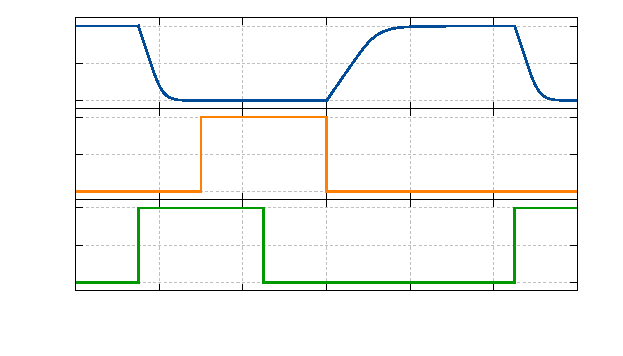
\includegraphics[width={283.40bp},height={155.90bp}]{Immagini/nor-dinamica}}%
    \gplfronttext
  \end{picture}%
\endgroup


		\caption{risposta del gate nor a due ingressi di onde quadre di periodi multipli. Come nel caso dell'invertitore (fig. \ref{fig:not:dinamica-schema}) il circuito a valle della porta logica è modellato da una capacità di carico di $0.75pF$.  Le tensioni sono espresse in volt.}
		\label{fig:nor:dinamica}
	\end{figure}

	Calcolando i tempi di propagazione dei segnali per un'escursione del $95\%$ della tensione di alimentazione, è possibile osservare che il tempo di transizione del segnale dal valore logico alto a quello basso è minore rispetto alla transizione inversa ($7.22ns$ vs $14.73 ns$): tale effetto è giustificabile considerando il fatto che la rete di pulldown composta dal parallelo di n-mos permette di generare una quantità di corrente maggiore rispetto alla rete di pull-up determinata dalla serie di p-mos. Un modo dunque per correggere questo sbilanciamento sarebbe di rideterminare dei nuovi parametri $W/L$ per i transistor in modo da bilanciare il comportamento.
	
	\begin{figure}[H]
		\centering
		% GNUPLOT: LaTeX picture with Postscript
\begingroup
  \makeatletter
  \providecommand\color[2][]{%
    \GenericError{(gnuplot) \space\space\space\@spaces}{%
      Package color not loaded in conjunction with
      terminal option `colourtext'%
    }{See the gnuplot documentation for explanation.%
    }{Either use 'blacktext' in gnuplot or load the package
      color.sty in LaTeX.}%
    \renewcommand\color[2][]{}%
  }%
  \providecommand\includegraphics[2][]{%
    \GenericError{(gnuplot) \space\space\space\@spaces}{%
      Package graphicx or graphics not loaded%
    }{See the gnuplot documentation for explanation.%
    }{The gnuplot epslatex terminal needs graphicx.sty or graphics.sty.}%
    \renewcommand\includegraphics[2][]{}%
  }%
  \providecommand\rotatebox[2]{#2}%
  \@ifundefined{ifGPcolor}{%
    \newif\ifGPcolor
    \GPcolorfalse
  }{}%
  \@ifundefined{ifGPblacktext}{%
    \newif\ifGPblacktext
    \GPblacktexttrue
  }{}%
  % define a \g@addto@macro without @ in the name:
  \let\gplgaddtomacro\g@addto@macro
  % define empty templates for all commands taking text:
  \gdef\gplbacktext{}%
  \gdef\gplfronttext{}%
  \makeatother
  \ifGPblacktext
    % no textcolor at all
    \def\colorrgb#1{}%
    \def\colorgray#1{}%
  \else
    % gray or color?
    \ifGPcolor
      \def\colorrgb#1{\color[rgb]{#1}}%
      \def\colorgray#1{\color[gray]{#1}}%
      \expandafter\def\csname LTw\endcsname{\color{white}}%
      \expandafter\def\csname LTb\endcsname{\color{black}}%
      \expandafter\def\csname LTa\endcsname{\color{black}}%
      \expandafter\def\csname LT0\endcsname{\color[rgb]{1,0,0}}%
      \expandafter\def\csname LT1\endcsname{\color[rgb]{0,1,0}}%
      \expandafter\def\csname LT2\endcsname{\color[rgb]{0,0,1}}%
      \expandafter\def\csname LT3\endcsname{\color[rgb]{1,0,1}}%
      \expandafter\def\csname LT4\endcsname{\color[rgb]{0,1,1}}%
      \expandafter\def\csname LT5\endcsname{\color[rgb]{1,1,0}}%
      \expandafter\def\csname LT6\endcsname{\color[rgb]{0,0,0}}%
      \expandafter\def\csname LT7\endcsname{\color[rgb]{1,0.3,0}}%
      \expandafter\def\csname LT8\endcsname{\color[rgb]{0.5,0.5,0.5}}%
    \else
      % gray
      \def\colorrgb#1{\color{black}}%
      \def\colorgray#1{\color[gray]{#1}}%
      \expandafter\def\csname LTw\endcsname{\color{white}}%
      \expandafter\def\csname LTb\endcsname{\color{black}}%
      \expandafter\def\csname LTa\endcsname{\color{black}}%
      \expandafter\def\csname LT0\endcsname{\color{black}}%
      \expandafter\def\csname LT1\endcsname{\color{black}}%
      \expandafter\def\csname LT2\endcsname{\color{black}}%
      \expandafter\def\csname LT3\endcsname{\color{black}}%
      \expandafter\def\csname LT4\endcsname{\color{black}}%
      \expandafter\def\csname LT5\endcsname{\color{black}}%
      \expandafter\def\csname LT6\endcsname{\color{black}}%
      \expandafter\def\csname LT7\endcsname{\color{black}}%
      \expandafter\def\csname LT8\endcsname{\color{black}}%
    \fi
  \fi
    \setlength{\unitlength}{0.0500bp}%
    \ifx\gptboxheight\undefined%
      \newlength{\gptboxheight}%
      \newlength{\gptboxwidth}%
      \newsavebox{\gptboxtext}%
    \fi%
    \setlength{\fboxrule}{0.5pt}%
    \setlength{\fboxsep}{1pt}%
\begin{picture}(5668.00,3118.00)%
    \gplgaddtomacro\gplbacktext{%
      \csname LTb\endcsname%%
      \put(434,2292){\makebox(0,0)[r]{\strut{}$0$}}%
      \csname LTb\endcsname%%
      \put(434,2649){\makebox(0,0)[r]{\strut{}$0.9$}}%
      \csname LTb\endcsname%%
      \put(434,3006){\makebox(0,0)[r]{\strut{}$1.8$}}%
      \csname LTb\endcsname%%
      \put(566,1993){\makebox(0,0){\strut{}}}%
      \csname LTb\endcsname%%
      \put(1101,1993){\makebox(0,0){\strut{}}}%
      \csname LTb\endcsname%%
      \put(1636,1993){\makebox(0,0){\strut{}}}%
      \csname LTb\endcsname%%
      \put(2172,1993){\makebox(0,0){\strut{}}}%
      \csname LTb\endcsname%%
      \put(2707,1993){\makebox(0,0){\strut{}}}%
      \csname LTb\endcsname%%
      \put(3242,1993){\makebox(0,0){\strut{}}}%
      \csname LTb\endcsname%%
      \put(3777,1993){\makebox(0,0){\strut{}}}%
      \csname LTb\endcsname%%
      \put(4313,1993){\makebox(0,0){\strut{}}}%
      \csname LTb\endcsname%%
      \put(4848,1993){\makebox(0,0){\strut{}}}%
      \csname LTb\endcsname%%
      \put(5383,1993){\makebox(0,0){\strut{}}}%
    }%
    \gplgaddtomacro\gplfronttext{%
      \csname LTb\endcsname%%
      \put(-171,2649){\rotatebox{-270}{\makebox(0,0){\strut{}$V_{out}$}}}%
      \put(2974,1927){\makebox(0,0){\strut{}}}%
    }%
    \gplgaddtomacro\gplbacktext{%
      \csname LTb\endcsname%%
      \put(434,1419){\makebox(0,0)[r]{\strut{}$0$}}%
      \csname LTb\endcsname%%
      \put(434,1777){\makebox(0,0)[r]{\strut{}$0.9$}}%
      \csname LTb\endcsname%%
      \put(434,2134){\makebox(0,0)[r]{\strut{}$1.8$}}%
      \csname LTb\endcsname%%
      \put(566,1120){\makebox(0,0){\strut{}}}%
      \csname LTb\endcsname%%
      \put(1101,1120){\makebox(0,0){\strut{}}}%
      \csname LTb\endcsname%%
      \put(1636,1120){\makebox(0,0){\strut{}}}%
      \csname LTb\endcsname%%
      \put(2172,1120){\makebox(0,0){\strut{}}}%
      \csname LTb\endcsname%%
      \put(2707,1120){\makebox(0,0){\strut{}}}%
      \csname LTb\endcsname%%
      \put(3242,1120){\makebox(0,0){\strut{}}}%
      \csname LTb\endcsname%%
      \put(3777,1120){\makebox(0,0){\strut{}}}%
      \csname LTb\endcsname%%
      \put(4313,1120){\makebox(0,0){\strut{}}}%
      \csname LTb\endcsname%%
      \put(4848,1120){\makebox(0,0){\strut{}}}%
      \csname LTb\endcsname%%
      \put(5383,1120){\makebox(0,0){\strut{}}}%
    }%
    \gplgaddtomacro\gplfronttext{%
      \csname LTb\endcsname%%
      \put(-171,1776){\rotatebox{-270}{\makebox(0,0){\strut{}$V_{in,1}$}}}%
      \put(2974,1054){\makebox(0,0){\strut{}}}%
    }%
    \gplgaddtomacro\gplbacktext{%
      \csname LTb\endcsname%%
      \put(434,546){\makebox(0,0)[r]{\strut{}$0$}}%
      \csname LTb\endcsname%%
      \put(434,904){\makebox(0,0)[r]{\strut{}$0.9$}}%
      \csname LTb\endcsname%%
      \put(434,1261){\makebox(0,0)[r]{\strut{}$1.8$}}%
      \csname LTb\endcsname%%
      \put(566,247){\makebox(0,0){\strut{}0}}%
      \csname LTb\endcsname%%
      \put(1101,247){\makebox(0,0){\strut{}10}}%
      \csname LTb\endcsname%%
      \put(1636,247){\makebox(0,0){\strut{}20}}%
      \csname LTb\endcsname%%
      \put(2172,247){\makebox(0,0){\strut{}30}}%
      \csname LTb\endcsname%%
      \put(2707,247){\makebox(0,0){\strut{}40}}%
      \csname LTb\endcsname%%
      \put(3242,247){\makebox(0,0){\strut{}50}}%
      \csname LTb\endcsname%%
      \put(3777,247){\makebox(0,0){\strut{}60}}%
      \csname LTb\endcsname%%
      \put(4313,247){\makebox(0,0){\strut{}70}}%
      \csname LTb\endcsname%%
      \put(4848,247){\makebox(0,0){\strut{}80}}%
      \csname LTb\endcsname%%
      \put(5383,247){\makebox(0,0){\strut{}90}}%
    }%
    \gplgaddtomacro\gplfronttext{%
      \csname LTb\endcsname%%
      \put(-171,903){\rotatebox{-270}{\makebox(0,0){\strut{}$V_{in,2}$}}}%
      \put(2974,-83){\makebox(0,0){\strut{}tempo $[ns]$}}%
    }%
    \gplbacktext
    \put(0,0){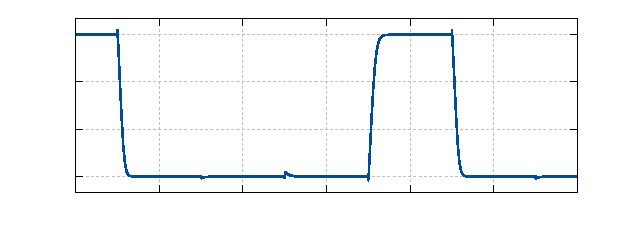
\includegraphics[width={283.40bp},height={155.90bp}]{Immagini/nor-dinamica-corr}}%
    \gplfronttext
  \end{picture}%
\endgroup


		\vspace{3.5mm}
		\caption{risposta del circuito nor ottenuta aumentando il rapporto $W/L$ dei p-mos al valore $4.8/0.15 \mu m/\mu m$; i mosfet a substrato n rimangono invarianti con un rapporto $1/0.45\mu m/\mu m$.  Le tensioni sono espresse in volt.}
		\label{fig:nor:dinamica-corretta}
	\end{figure}
	
	Diminuendo la larghezza $W$ dei transistor p-mos al valore $0.15\mu m$ il comportamento del circuito tende a bilanciarsi (come si può osservare in figura \ref{fig:nor:dinamica-corretta}), con tempi di transizione da uscita alta a bassa di $3.61ns$ e da uscita bassa ad alta di $4.31ns$. 
	
\section{Nand gate}
	La porta logica \textit{nand}, coincidente con la negazione del gate \textit{and}, è il gate che, per costruzione, risulta duale alla porta nor appena studiata ed è caratterizzata dalla tabella di verità
	\begin{center}
		\begin{tabular}{c c | c}
			$V_{in,1}$ & $V_{in,2}$ & $V_{out}$ \\ \hline
			0 & 0 & 1 \\
			0 & 1 & 1 \\
			1 & 0 & 1 \\
			1 & 1 & 0 \\
		\end{tabular}
	\end{center}
	
	La realizzazione circuitale della porta logica, come in figura \ref{fig:nand:schematico}, è molto simile al gate nor, dove tuttavia la rete di pull-up è realizzata da un parallelo (e non da una serie) di p-mos, mentre la rete di pull-down è realizzata da una serie (e non da un parallelo) di transistor n-mos. Avendo osservato l'asimmetria di comportamento dovuta al collegamento in serie/parallelo dei mosfet vista nel gate nor, si procede sin da principio a diminuire la larghezza $W$ degli n-mos al valore di $0.15 \mu m$.

	\begin{figure}[bht]
		\centering
		\begin{subfigure}{0.48\linewidth}
			\centering
			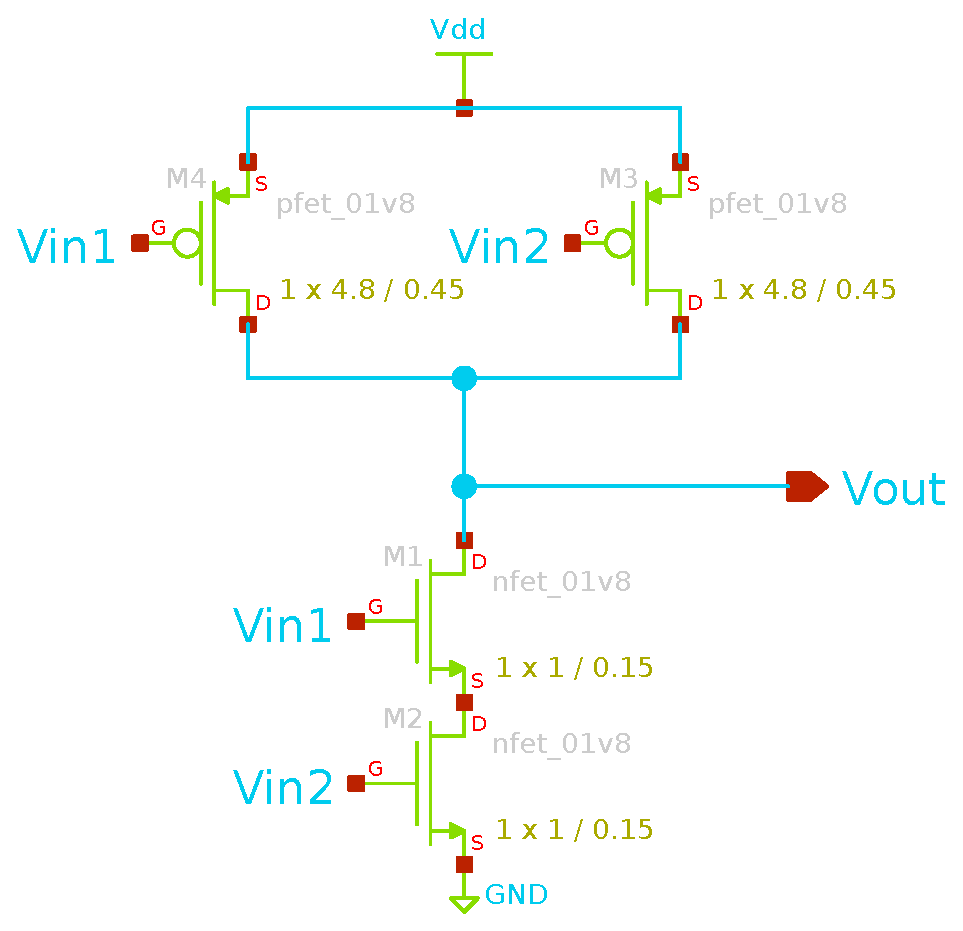
\includegraphics[width=5cm]{Immagini/nand-gate.eps} \caption{}			
		\end{subfigure}
		\begin{subfigure}{0.48\linewidth}
			\centering
			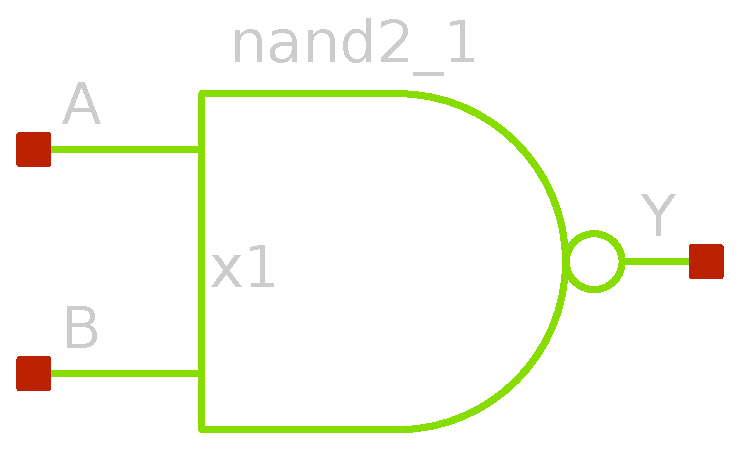
\includegraphics[width=2.5cm]{Immagini/nand-gate-simple.eps} \caption{}			
		\end{subfigure}
		\caption{implementazione della porta logica nand in tecnologia c-mos (a) e la relativa rappresentazione schematica (b).}
		\label{fig:nand:schematico}
	\end{figure}

	Il funzionamento del circuito può essere analizzato studiando le possibili combinazioni dei segnali in ingresso:
	\begin{itemize}
		\item nel caso in cui entrambi i segnali si trovino ad un valore logico alto (quarta riga della tabella di verità) la rete di pull-up risulterebbe interdetta (entrambi i p-mos sono spenti per via della tensione $V_{gs}$ nulla), mentre la rete di pull-down a transistor accesi permette un passaggio di corrente. Dovendo la stessa essere nulla per il bilancio della corrente al nodo d'uscita, si osserva necessariamente che $V_{out} = 0$;
		
		\item in tutti gli altri casi in cui almeno un ingresso sia allo stato logico basso, allora sicuramente uno degli n-mos sarebbe interdetto (e dunque di conseguenza lo è anche la rete di pull-down), mentre almeno uno dei p-mos rimarrebbe accesso, permettendo il passaggio di corrente nella rete di pull-up. Il bilancio della corrente al nodo d'uscita permette infine di stabilire che il relativo stato logico è alto ($V_{out} = V_{dd}$). 
	\end{itemize}

	Mediante una simulazione del transitorio nel tempo (con capacità di carico di $0.75pF$) è dunque possibile verificare il comportamento logico del circuito, arrivando ai risultati mostrati in figura \ref{fig:nand:dinamica}.	

	\begin{figure}[bht]
		\centering
		% GNUPLOT: LaTeX picture with Postscript
\begingroup
  \makeatletter
  \providecommand\color[2][]{%
    \GenericError{(gnuplot) \space\space\space\@spaces}{%
      Package color not loaded in conjunction with
      terminal option `colourtext'%
    }{See the gnuplot documentation for explanation.%
    }{Either use 'blacktext' in gnuplot or load the package
      color.sty in LaTeX.}%
    \renewcommand\color[2][]{}%
  }%
  \providecommand\includegraphics[2][]{%
    \GenericError{(gnuplot) \space\space\space\@spaces}{%
      Package graphicx or graphics not loaded%
    }{See the gnuplot documentation for explanation.%
    }{The gnuplot epslatex terminal needs graphicx.sty or graphics.sty.}%
    \renewcommand\includegraphics[2][]{}%
  }%
  \providecommand\rotatebox[2]{#2}%
  \@ifundefined{ifGPcolor}{%
    \newif\ifGPcolor
    \GPcolorfalse
  }{}%
  \@ifundefined{ifGPblacktext}{%
    \newif\ifGPblacktext
    \GPblacktexttrue
  }{}%
  % define a \g@addto@macro without @ in the name:
  \let\gplgaddtomacro\g@addto@macro
  % define empty templates for all commands taking text:
  \gdef\gplbacktext{}%
  \gdef\gplfronttext{}%
  \makeatother
  \ifGPblacktext
    % no textcolor at all
    \def\colorrgb#1{}%
    \def\colorgray#1{}%
  \else
    % gray or color?
    \ifGPcolor
      \def\colorrgb#1{\color[rgb]{#1}}%
      \def\colorgray#1{\color[gray]{#1}}%
      \expandafter\def\csname LTw\endcsname{\color{white}}%
      \expandafter\def\csname LTb\endcsname{\color{black}}%
      \expandafter\def\csname LTa\endcsname{\color{black}}%
      \expandafter\def\csname LT0\endcsname{\color[rgb]{1,0,0}}%
      \expandafter\def\csname LT1\endcsname{\color[rgb]{0,1,0}}%
      \expandafter\def\csname LT2\endcsname{\color[rgb]{0,0,1}}%
      \expandafter\def\csname LT3\endcsname{\color[rgb]{1,0,1}}%
      \expandafter\def\csname LT4\endcsname{\color[rgb]{0,1,1}}%
      \expandafter\def\csname LT5\endcsname{\color[rgb]{1,1,0}}%
      \expandafter\def\csname LT6\endcsname{\color[rgb]{0,0,0}}%
      \expandafter\def\csname LT7\endcsname{\color[rgb]{1,0.3,0}}%
      \expandafter\def\csname LT8\endcsname{\color[rgb]{0.5,0.5,0.5}}%
    \else
      % gray
      \def\colorrgb#1{\color{black}}%
      \def\colorgray#1{\color[gray]{#1}}%
      \expandafter\def\csname LTw\endcsname{\color{white}}%
      \expandafter\def\csname LTb\endcsname{\color{black}}%
      \expandafter\def\csname LTa\endcsname{\color{black}}%
      \expandafter\def\csname LT0\endcsname{\color{black}}%
      \expandafter\def\csname LT1\endcsname{\color{black}}%
      \expandafter\def\csname LT2\endcsname{\color{black}}%
      \expandafter\def\csname LT3\endcsname{\color{black}}%
      \expandafter\def\csname LT4\endcsname{\color{black}}%
      \expandafter\def\csname LT5\endcsname{\color{black}}%
      \expandafter\def\csname LT6\endcsname{\color{black}}%
      \expandafter\def\csname LT7\endcsname{\color{black}}%
      \expandafter\def\csname LT8\endcsname{\color{black}}%
    \fi
  \fi
    \setlength{\unitlength}{0.0500bp}%
    \ifx\gptboxheight\undefined%
      \newlength{\gptboxheight}%
      \newlength{\gptboxwidth}%
      \newsavebox{\gptboxtext}%
    \fi%
    \setlength{\fboxrule}{0.5pt}%
    \setlength{\fboxsep}{1pt}%
\begin{picture}(5668.00,3118.00)%
    \gplgaddtomacro\gplbacktext{%
      \csname LTb\endcsname%%
      \put(434,2292){\makebox(0,0)[r]{\strut{}$0$}}%
      \csname LTb\endcsname%%
      \put(434,2649){\makebox(0,0)[r]{\strut{}$0.9$}}%
      \csname LTb\endcsname%%
      \put(434,3006){\makebox(0,0)[r]{\strut{}$1.8$}}%
      \csname LTb\endcsname%%
      \put(566,1993){\makebox(0,0){\strut{}}}%
      \csname LTb\endcsname%%
      \put(1101,1993){\makebox(0,0){\strut{}}}%
      \csname LTb\endcsname%%
      \put(1636,1993){\makebox(0,0){\strut{}}}%
      \csname LTb\endcsname%%
      \put(2172,1993){\makebox(0,0){\strut{}}}%
      \csname LTb\endcsname%%
      \put(2707,1993){\makebox(0,0){\strut{}}}%
      \csname LTb\endcsname%%
      \put(3242,1993){\makebox(0,0){\strut{}}}%
      \csname LTb\endcsname%%
      \put(3777,1993){\makebox(0,0){\strut{}}}%
      \csname LTb\endcsname%%
      \put(4313,1993){\makebox(0,0){\strut{}}}%
      \csname LTb\endcsname%%
      \put(4848,1993){\makebox(0,0){\strut{}}}%
      \csname LTb\endcsname%%
      \put(5383,1993){\makebox(0,0){\strut{}}}%
    }%
    \gplgaddtomacro\gplfronttext{%
      \csname LTb\endcsname%%
      \put(-171,2649){\rotatebox{-270}{\makebox(0,0){\strut{}$V_{out}$}}}%
      \put(2974,1927){\makebox(0,0){\strut{}}}%
    }%
    \gplgaddtomacro\gplbacktext{%
      \csname LTb\endcsname%%
      \put(434,1419){\makebox(0,0)[r]{\strut{}$0$}}%
      \csname LTb\endcsname%%
      \put(434,1777){\makebox(0,0)[r]{\strut{}$0.9$}}%
      \csname LTb\endcsname%%
      \put(434,2134){\makebox(0,0)[r]{\strut{}$1.8$}}%
      \csname LTb\endcsname%%
      \put(566,1120){\makebox(0,0){\strut{}}}%
      \csname LTb\endcsname%%
      \put(1101,1120){\makebox(0,0){\strut{}}}%
      \csname LTb\endcsname%%
      \put(1636,1120){\makebox(0,0){\strut{}}}%
      \csname LTb\endcsname%%
      \put(2172,1120){\makebox(0,0){\strut{}}}%
      \csname LTb\endcsname%%
      \put(2707,1120){\makebox(0,0){\strut{}}}%
      \csname LTb\endcsname%%
      \put(3242,1120){\makebox(0,0){\strut{}}}%
      \csname LTb\endcsname%%
      \put(3777,1120){\makebox(0,0){\strut{}}}%
      \csname LTb\endcsname%%
      \put(4313,1120){\makebox(0,0){\strut{}}}%
      \csname LTb\endcsname%%
      \put(4848,1120){\makebox(0,0){\strut{}}}%
      \csname LTb\endcsname%%
      \put(5383,1120){\makebox(0,0){\strut{}}}%
    }%
    \gplgaddtomacro\gplfronttext{%
      \csname LTb\endcsname%%
      \put(-171,1776){\rotatebox{-270}{\makebox(0,0){\strut{}$V_{in,1}$}}}%
      \put(2974,1054){\makebox(0,0){\strut{}}}%
    }%
    \gplgaddtomacro\gplbacktext{%
      \csname LTb\endcsname%%
      \put(434,546){\makebox(0,0)[r]{\strut{}$0$}}%
      \csname LTb\endcsname%%
      \put(434,904){\makebox(0,0)[r]{\strut{}$0.9$}}%
      \csname LTb\endcsname%%
      \put(434,1261){\makebox(0,0)[r]{\strut{}$1.8$}}%
      \csname LTb\endcsname%%
      \put(566,247){\makebox(0,0){\strut{}0}}%
      \csname LTb\endcsname%%
      \put(1101,247){\makebox(0,0){\strut{}10}}%
      \csname LTb\endcsname%%
      \put(1636,247){\makebox(0,0){\strut{}20}}%
      \csname LTb\endcsname%%
      \put(2172,247){\makebox(0,0){\strut{}30}}%
      \csname LTb\endcsname%%
      \put(2707,247){\makebox(0,0){\strut{}40}}%
      \csname LTb\endcsname%%
      \put(3242,247){\makebox(0,0){\strut{}50}}%
      \csname LTb\endcsname%%
      \put(3777,247){\makebox(0,0){\strut{}60}}%
      \csname LTb\endcsname%%
      \put(4313,247){\makebox(0,0){\strut{}70}}%
      \csname LTb\endcsname%%
      \put(4848,247){\makebox(0,0){\strut{}80}}%
      \csname LTb\endcsname%%
      \put(5383,247){\makebox(0,0){\strut{}90}}%
    }%
    \gplgaddtomacro\gplfronttext{%
      \csname LTb\endcsname%%
      \put(-171,903){\rotatebox{-270}{\makebox(0,0){\strut{}$V_{in,2}$}}}%
      \put(2974,-83){\makebox(0,0){\strut{}tempo $[ns]$}}%
    }%
    \gplbacktext
    \put(0,0){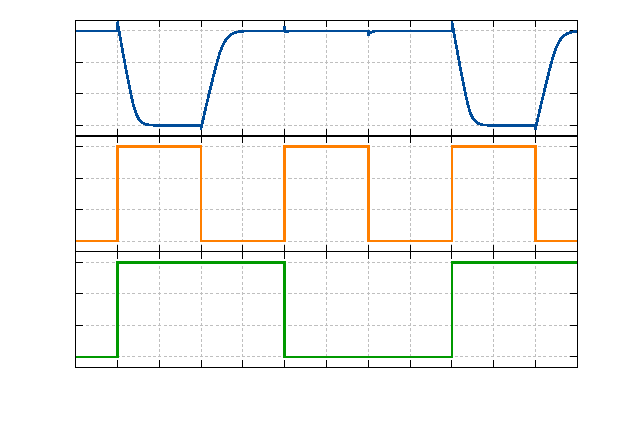
\includegraphics[width={283.40bp},height={155.90bp}]{Immagini/nand-dinamica}}%
    \gplfronttext
  \end{picture}%
\endgroup

		\caption{risposta del gate nand a due ingressi di onde quadre di periodi multipli. Come nel caso dell'invertitore (fig. \ref{fig:not:dinamica-schema}) il circuito a valle della porta logica è modellato da una capacità di carico di $0.75pF$.  Le tensioni sono espresse in volt.}
		\label{fig:nand:dinamica}
	\end{figure}
	
	A questo punto è possibile misurare il tempo di commutazione dell'uscita nel passaggio da tensione alta a bassa (misurata al $95\%$ dell'escursione del segnale), che si attesta al valore di $5.51ns$, mentre il passaggio del segnale da basso ad alto dura $7.14ns$.
	
\section{And \& or gate}
	Avendo studiato singolarmente i gate nand, nor e not, la costruzione dei gate logici \textit{and} e \textit{or} deriva direttamente tramite la connessione in sequenza della rispettiva porta negata con l'invertitore logico. In particolare le tabelle di verità che i due componenti devono realizzare sono:
	
	\begin{center}
		\begin{tabular}{c c | c | c}
			$V_{in,1}$ & $V_{in,2}$ & $V_{out,and}$ & $V_{out,or}$ \\ \hline
			0 & 0 & 0 & 0 \\
			0 & 1 & 0 & 1 \\
			1 & 0 & 0 & 1 \\
			1 & 1 & 1 & 1 \\
		\end{tabular}
	\end{center}

	\begin{figure}[bht]
		\centering
		\begin{subfigure}{0.48\linewidth}
			\centering 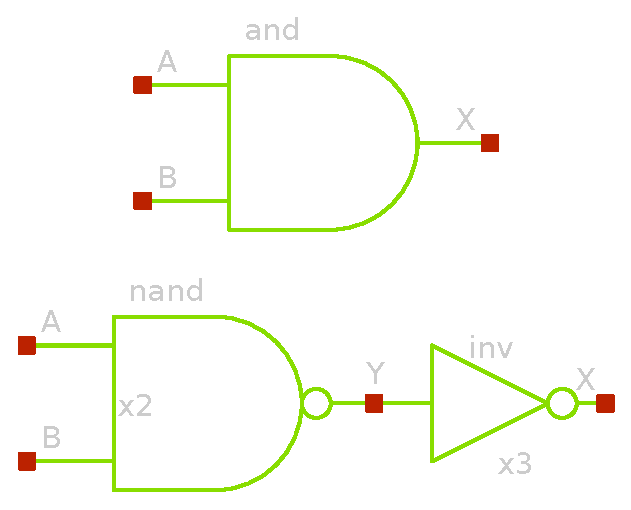
\includegraphics[width=4cm]{Immagini/and-simple} \caption{}
		\end{subfigure}
		\begin{subfigure}{0.48\linewidth}
			\centering 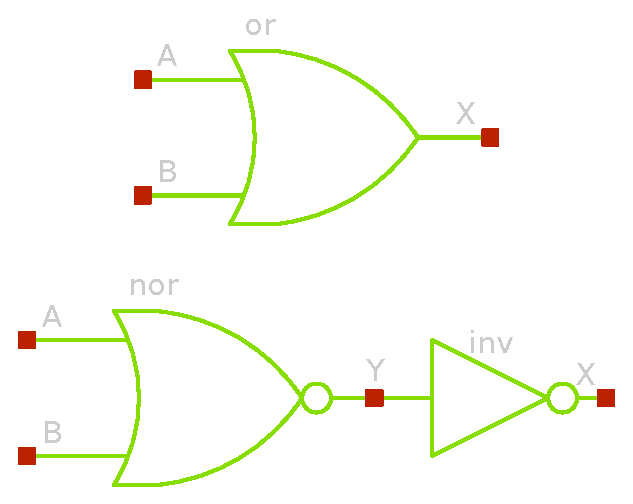
\includegraphics[width=4cm]{Immagini/or-simple} \caption{}
		\end{subfigure}
		\caption{rappresentazione schematica (sopra) e blocchi elementari che costituiscono (sotto) i gate logici and (a) e or (b).}
		\label{fig:andor:simbolo}
	\end{figure}
	
	In figura \ref{fig:andor:simbolo} si osserva la rappresentazione semplificata delle porte logiche che espandendone le implementazioni in tecnologia c-mos determinano gli schematici riportati in figura \ref{fig:andor:schematico}.
	
	\begin{figure}[bht]
	\centering
	\begin{subfigure}{0.48\linewidth}
		\centering 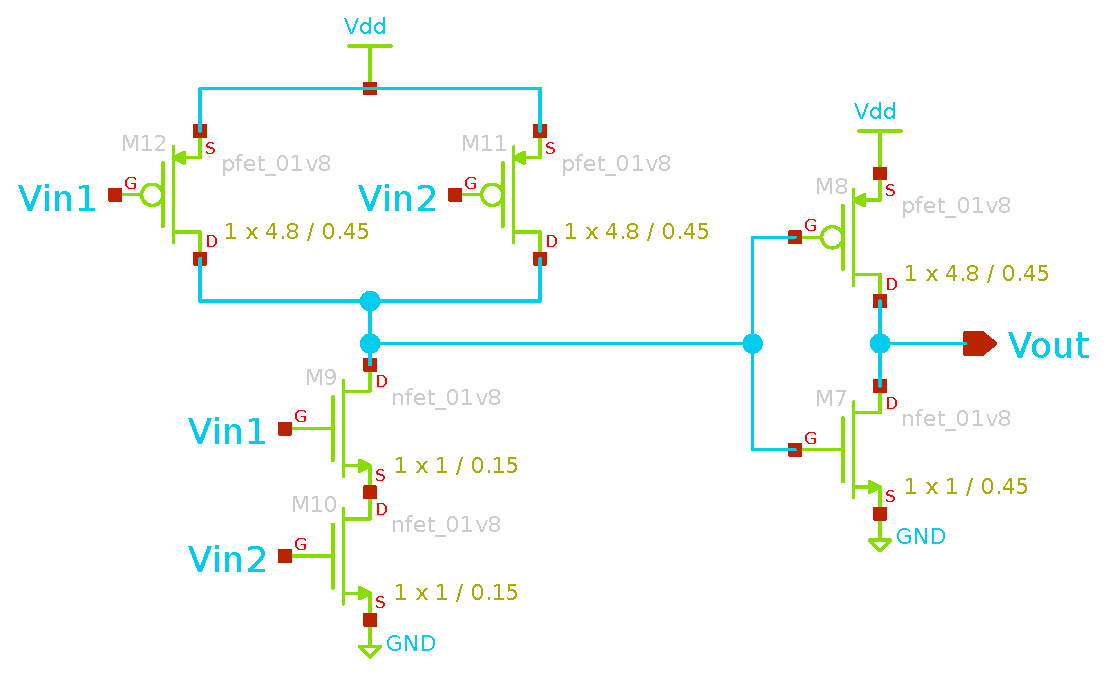
\includegraphics[width=0.9\linewidth]{Immagini/and-gate} \caption{}
	\end{subfigure}
	\begin{subfigure}{0.48\linewidth}
		\centering 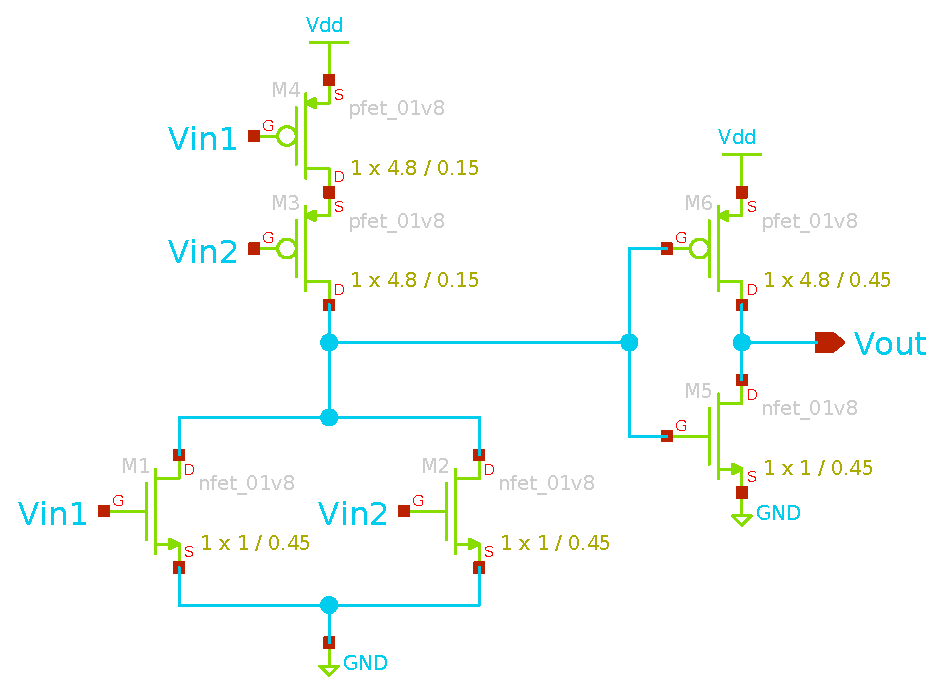
\includegraphics[width=0.9\linewidth]{Immagini/or-gate} \caption{}
	\end{subfigure}
	\caption{implementazione in tecnlogia c-mos della porta logica and (a) e or (b).}
	\label{fig:andor:schematico}
	\end{figure}

	E' inoltre possibile procedere con le simulazioni dei transitori (con una capacità di carico di $0.75pF$) che determinano gli andamenti temporali mostrati in figura \ref{fig:andor:dinamica}. Analizzando i tempi di propagazione dei segnali all'interno dei circuiti si arriva a dei tempi massimi per i due circuiti che si attestano ai valori
	\[ \tau_{max,and} \approx 7.31 ns \qquad \tau_{max,or} \approx 7.21 ns  \]


	\begin{figure}[bht]
		\centering
		% GNUPLOT: LaTeX picture with Postscript
\begingroup
  \makeatletter
  \providecommand\color[2][]{%
    \GenericError{(gnuplot) \space\space\space\@spaces}{%
      Package color not loaded in conjunction with
      terminal option `colourtext'%
    }{See the gnuplot documentation for explanation.%
    }{Either use 'blacktext' in gnuplot or load the package
      color.sty in LaTeX.}%
    \renewcommand\color[2][]{}%
  }%
  \providecommand\includegraphics[2][]{%
    \GenericError{(gnuplot) \space\space\space\@spaces}{%
      Package graphicx or graphics not loaded%
    }{See the gnuplot documentation for explanation.%
    }{The gnuplot epslatex terminal needs graphicx.sty or graphics.sty.}%
    \renewcommand\includegraphics[2][]{}%
  }%
  \providecommand\rotatebox[2]{#2}%
  \@ifundefined{ifGPcolor}{%
    \newif\ifGPcolor
    \GPcolorfalse
  }{}%
  \@ifundefined{ifGPblacktext}{%
    \newif\ifGPblacktext
    \GPblacktexttrue
  }{}%
  % define a \g@addto@macro without @ in the name:
  \let\gplgaddtomacro\g@addto@macro
  % define empty templates for all commands taking text:
  \gdef\gplbacktext{}%
  \gdef\gplfronttext{}%
  \makeatother
  \ifGPblacktext
    % no textcolor at all
    \def\colorrgb#1{}%
    \def\colorgray#1{}%
  \else
    % gray or color?
    \ifGPcolor
      \def\colorrgb#1{\color[rgb]{#1}}%
      \def\colorgray#1{\color[gray]{#1}}%
      \expandafter\def\csname LTw\endcsname{\color{white}}%
      \expandafter\def\csname LTb\endcsname{\color{black}}%
      \expandafter\def\csname LTa\endcsname{\color{black}}%
      \expandafter\def\csname LT0\endcsname{\color[rgb]{1,0,0}}%
      \expandafter\def\csname LT1\endcsname{\color[rgb]{0,1,0}}%
      \expandafter\def\csname LT2\endcsname{\color[rgb]{0,0,1}}%
      \expandafter\def\csname LT3\endcsname{\color[rgb]{1,0,1}}%
      \expandafter\def\csname LT4\endcsname{\color[rgb]{0,1,1}}%
      \expandafter\def\csname LT5\endcsname{\color[rgb]{1,1,0}}%
      \expandafter\def\csname LT6\endcsname{\color[rgb]{0,0,0}}%
      \expandafter\def\csname LT7\endcsname{\color[rgb]{1,0.3,0}}%
      \expandafter\def\csname LT8\endcsname{\color[rgb]{0.5,0.5,0.5}}%
    \else
      % gray
      \def\colorrgb#1{\color{black}}%
      \def\colorgray#1{\color[gray]{#1}}%
      \expandafter\def\csname LTw\endcsname{\color{white}}%
      \expandafter\def\csname LTb\endcsname{\color{black}}%
      \expandafter\def\csname LTa\endcsname{\color{black}}%
      \expandafter\def\csname LT0\endcsname{\color{black}}%
      \expandafter\def\csname LT1\endcsname{\color{black}}%
      \expandafter\def\csname LT2\endcsname{\color{black}}%
      \expandafter\def\csname LT3\endcsname{\color{black}}%
      \expandafter\def\csname LT4\endcsname{\color{black}}%
      \expandafter\def\csname LT5\endcsname{\color{black}}%
      \expandafter\def\csname LT6\endcsname{\color{black}}%
      \expandafter\def\csname LT7\endcsname{\color{black}}%
      \expandafter\def\csname LT8\endcsname{\color{black}}%
    \fi
  \fi
    \setlength{\unitlength}{0.0500bp}%
    \ifx\gptboxheight\undefined%
      \newlength{\gptboxheight}%
      \newlength{\gptboxwidth}%
      \newsavebox{\gptboxtext}%
    \fi%
    \setlength{\fboxrule}{0.5pt}%
    \setlength{\fboxsep}{1pt}%
\begin{picture}(5668.00,5102.00)%
    \gplgaddtomacro\gplbacktext{%
      \csname LTb\endcsname%%
      \put(434,4076){\makebox(0,0)[r]{\strut{}$0$}}%
      \csname LTb\endcsname%%
      \put(434,4368){\makebox(0,0)[r]{\strut{}$0.6$}}%
      \csname LTb\endcsname%%
      \put(434,4660){\makebox(0,0)[r]{\strut{}$1.2$}}%
      \csname LTb\endcsname%%
      \put(434,4952){\makebox(0,0)[r]{\strut{}$1.8$}}%
      \csname LTb\endcsname%%
      \put(566,3759){\makebox(0,0){\strut{}}}%
      \csname LTb\endcsname%%
      \put(967,3759){\makebox(0,0){\strut{}}}%
      \csname LTb\endcsname%%
      \put(1369,3759){\makebox(0,0){\strut{}}}%
      \csname LTb\endcsname%%
      \put(1770,3759){\makebox(0,0){\strut{}}}%
      \csname LTb\endcsname%%
      \put(2172,3759){\makebox(0,0){\strut{}}}%
      \csname LTb\endcsname%%
      \put(2573,3759){\makebox(0,0){\strut{}}}%
      \csname LTb\endcsname%%
      \put(2975,3759){\makebox(0,0){\strut{}}}%
      \csname LTb\endcsname%%
      \put(3376,3759){\makebox(0,0){\strut{}}}%
      \csname LTb\endcsname%%
      \put(3777,3759){\makebox(0,0){\strut{}}}%
      \csname LTb\endcsname%%
      \put(4179,3759){\makebox(0,0){\strut{}}}%
      \csname LTb\endcsname%%
      \put(4580,3759){\makebox(0,0){\strut{}}}%
      \csname LTb\endcsname%%
      \put(4982,3759){\makebox(0,0){\strut{}}}%
      \csname LTb\endcsname%%
      \put(5383,3759){\makebox(0,0){\strut{}}}%
    }%
    \gplgaddtomacro\gplfronttext{%
      \csname LTb\endcsname%%
      \put(-171,4514){\rotatebox{-270}{\makebox(0,0){\strut{}$V_{out,and}$ $[V]$}}}%
      \put(2974,3693){\makebox(0,0){\strut{}}}%
    }%
    \gplgaddtomacro\gplbacktext{%
      \csname LTb\endcsname%%
      \put(434,3005){\makebox(0,0)[r]{\strut{}$0$}}%
      \csname LTb\endcsname%%
      \put(434,3297){\makebox(0,0)[r]{\strut{}$0.6$}}%
      \csname LTb\endcsname%%
      \put(434,3589){\makebox(0,0)[r]{\strut{}$1.2$}}%
      \csname LTb\endcsname%%
      \put(434,3881){\makebox(0,0)[r]{\strut{}$1.8$}}%
      \csname LTb\endcsname%%
      \put(566,2688){\makebox(0,0){\strut{}}}%
      \csname LTb\endcsname%%
      \put(967,2688){\makebox(0,0){\strut{}}}%
      \csname LTb\endcsname%%
      \put(1369,2688){\makebox(0,0){\strut{}}}%
      \csname LTb\endcsname%%
      \put(1770,2688){\makebox(0,0){\strut{}}}%
      \csname LTb\endcsname%%
      \put(2172,2688){\makebox(0,0){\strut{}}}%
      \csname LTb\endcsname%%
      \put(2573,2688){\makebox(0,0){\strut{}}}%
      \csname LTb\endcsname%%
      \put(2975,2688){\makebox(0,0){\strut{}}}%
      \csname LTb\endcsname%%
      \put(3376,2688){\makebox(0,0){\strut{}}}%
      \csname LTb\endcsname%%
      \put(3777,2688){\makebox(0,0){\strut{}}}%
      \csname LTb\endcsname%%
      \put(4179,2688){\makebox(0,0){\strut{}}}%
      \csname LTb\endcsname%%
      \put(4580,2688){\makebox(0,0){\strut{}}}%
      \csname LTb\endcsname%%
      \put(4982,2688){\makebox(0,0){\strut{}}}%
      \csname LTb\endcsname%%
      \put(5383,2688){\makebox(0,0){\strut{}}}%
    }%
    \gplgaddtomacro\gplfronttext{%
      \csname LTb\endcsname%%
      \put(-171,3443){\rotatebox{-270}{\makebox(0,0){\strut{}$V_{out,or}$ $[V]$}}}%
      \put(2974,2622){\makebox(0,0){\strut{}}}%
    }%
    \gplgaddtomacro\gplbacktext{%
      \csname LTb\endcsname%%
      \put(434,1933){\makebox(0,0)[r]{\strut{}$0$}}%
      \csname LTb\endcsname%%
      \put(434,2225){\makebox(0,0)[r]{\strut{}$0.6$}}%
      \csname LTb\endcsname%%
      \put(434,2518){\makebox(0,0)[r]{\strut{}$1.2$}}%
      \csname LTb\endcsname%%
      \put(434,2810){\makebox(0,0)[r]{\strut{}$1.8$}}%
      \csname LTb\endcsname%%
      \put(566,1616){\makebox(0,0){\strut{}}}%
      \csname LTb\endcsname%%
      \put(967,1616){\makebox(0,0){\strut{}}}%
      \csname LTb\endcsname%%
      \put(1369,1616){\makebox(0,0){\strut{}}}%
      \csname LTb\endcsname%%
      \put(1770,1616){\makebox(0,0){\strut{}}}%
      \csname LTb\endcsname%%
      \put(2172,1616){\makebox(0,0){\strut{}}}%
      \csname LTb\endcsname%%
      \put(2573,1616){\makebox(0,0){\strut{}}}%
      \csname LTb\endcsname%%
      \put(2975,1616){\makebox(0,0){\strut{}}}%
      \csname LTb\endcsname%%
      \put(3376,1616){\makebox(0,0){\strut{}}}%
      \csname LTb\endcsname%%
      \put(3777,1616){\makebox(0,0){\strut{}}}%
      \csname LTb\endcsname%%
      \put(4179,1616){\makebox(0,0){\strut{}}}%
      \csname LTb\endcsname%%
      \put(4580,1616){\makebox(0,0){\strut{}}}%
      \csname LTb\endcsname%%
      \put(4982,1616){\makebox(0,0){\strut{}}}%
      \csname LTb\endcsname%%
      \put(5383,1616){\makebox(0,0){\strut{}}}%
    }%
    \gplgaddtomacro\gplfronttext{%
      \csname LTb\endcsname%%
      \put(-171,2371){\rotatebox{-270}{\makebox(0,0){\strut{}$V_{in,1}$ $[V]$}}}%
      \put(2974,1550){\makebox(0,0){\strut{}}}%
    }%
    \gplgaddtomacro\gplbacktext{%
      \csname LTb\endcsname%%
      \put(434,862){\makebox(0,0)[r]{\strut{}$0$}}%
      \csname LTb\endcsname%%
      \put(434,1154){\makebox(0,0)[r]{\strut{}$0.6$}}%
      \csname LTb\endcsname%%
      \put(434,1447){\makebox(0,0)[r]{\strut{}$1.2$}}%
      \csname LTb\endcsname%%
      \put(434,1739){\makebox(0,0)[r]{\strut{}$1.8$}}%
      \csname LTb\endcsname%%
      \put(566,545){\makebox(0,0){\strut{}0}}%
      \csname LTb\endcsname%%
      \put(967,545){\makebox(0,0){\strut{}1.5}}%
      \csname LTb\endcsname%%
      \put(1369,545){\makebox(0,0){\strut{}3}}%
      \csname LTb\endcsname%%
      \put(1770,545){\makebox(0,0){\strut{}4.5}}%
      \csname LTb\endcsname%%
      \put(2172,545){\makebox(0,0){\strut{}6}}%
      \csname LTb\endcsname%%
      \put(2573,545){\makebox(0,0){\strut{}7.5}}%
      \csname LTb\endcsname%%
      \put(2975,545){\makebox(0,0){\strut{}9}}%
      \csname LTb\endcsname%%
      \put(3376,545){\makebox(0,0){\strut{}10.5}}%
      \csname LTb\endcsname%%
      \put(3777,545){\makebox(0,0){\strut{}12}}%
      \csname LTb\endcsname%%
      \put(4179,545){\makebox(0,0){\strut{}13.5}}%
      \csname LTb\endcsname%%
      \put(4580,545){\makebox(0,0){\strut{}15}}%
      \csname LTb\endcsname%%
      \put(4982,545){\makebox(0,0){\strut{}16.5}}%
      \csname LTb\endcsname%%
      \put(5383,545){\makebox(0,0){\strut{}18}}%
    }%
    \gplgaddtomacro\gplfronttext{%
      \csname LTb\endcsname%%
      \put(-171,1300){\rotatebox{-270}{\makebox(0,0){\strut{}$V_{in,2}$ $[V]$}}}%
      \put(2974,215){\makebox(0,0){\strut{}tempo $[ns]$}}%
    }%
    \gplbacktext
    \put(0,0){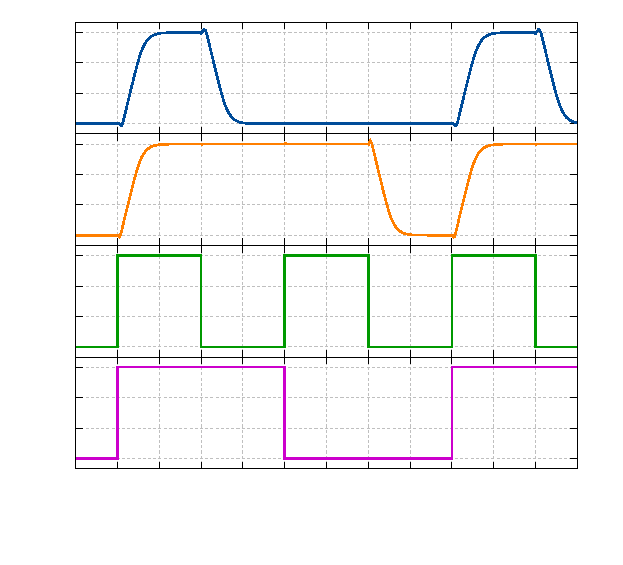
\includegraphics[width={283.40bp},height={255.10bp}]{Immagini/and-or-dinamica}}%
    \gplfronttext
  \end{picture}%
\endgroup


		\caption{risposta dei gate and e or a ingressi di onde quadre a periodi multipli. Come nel caso dell'invertitore (fig. \ref{fig:not:dinamica-schema}) il circuito a valle della porta logica è modellato da una capacità di carico di $0.75pF$. Le tensioni sono espresse in volt.}
		\label{fig:andor:dinamica}
	\end{figure}

\subsection*{Xor gate}
	Un'altra porta logica che verrà utilizzato nello sviluppo di alcuni circuiti combinatori è il gate logico \textit{xor}, ossia l'or esclusivo, per il quale l'uscita è alta solamente se uno degli ingressi è alto, ossia mediante rispettando la tabella di verità
	\begin{center}
		\begin{tabular}{c c | c}
			$V_{in,1}$ & $V_{in,2}$ & $V_{out}$ \\ \hline
			0 & 0 & 0 \\
			0 & 1 & 1 \\
			1 & 0 & 1 \\
			1 & 1 & 0 \\
		\end{tabular}
	\end{center}
	
	In figura \ref{fig:xor} è mostrata la rappresentazione schematica del gate logico xor mediante l'interconnessione di porte logiche precedentemente studiate.
	
	\begin{figure}[bht]
		\centering
		\begin{subfigure}{0.48\linewidth}
			\centering
			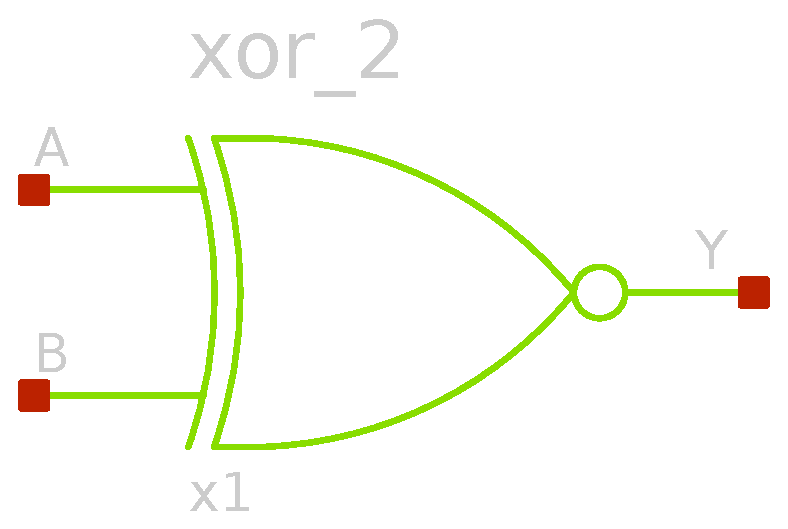
\includegraphics[width=3cm]{Immagini/xor-gate-simple}
			\caption{}
		\end{subfigure}
		\begin{subfigure}{0.48\linewidth}
			\centering
			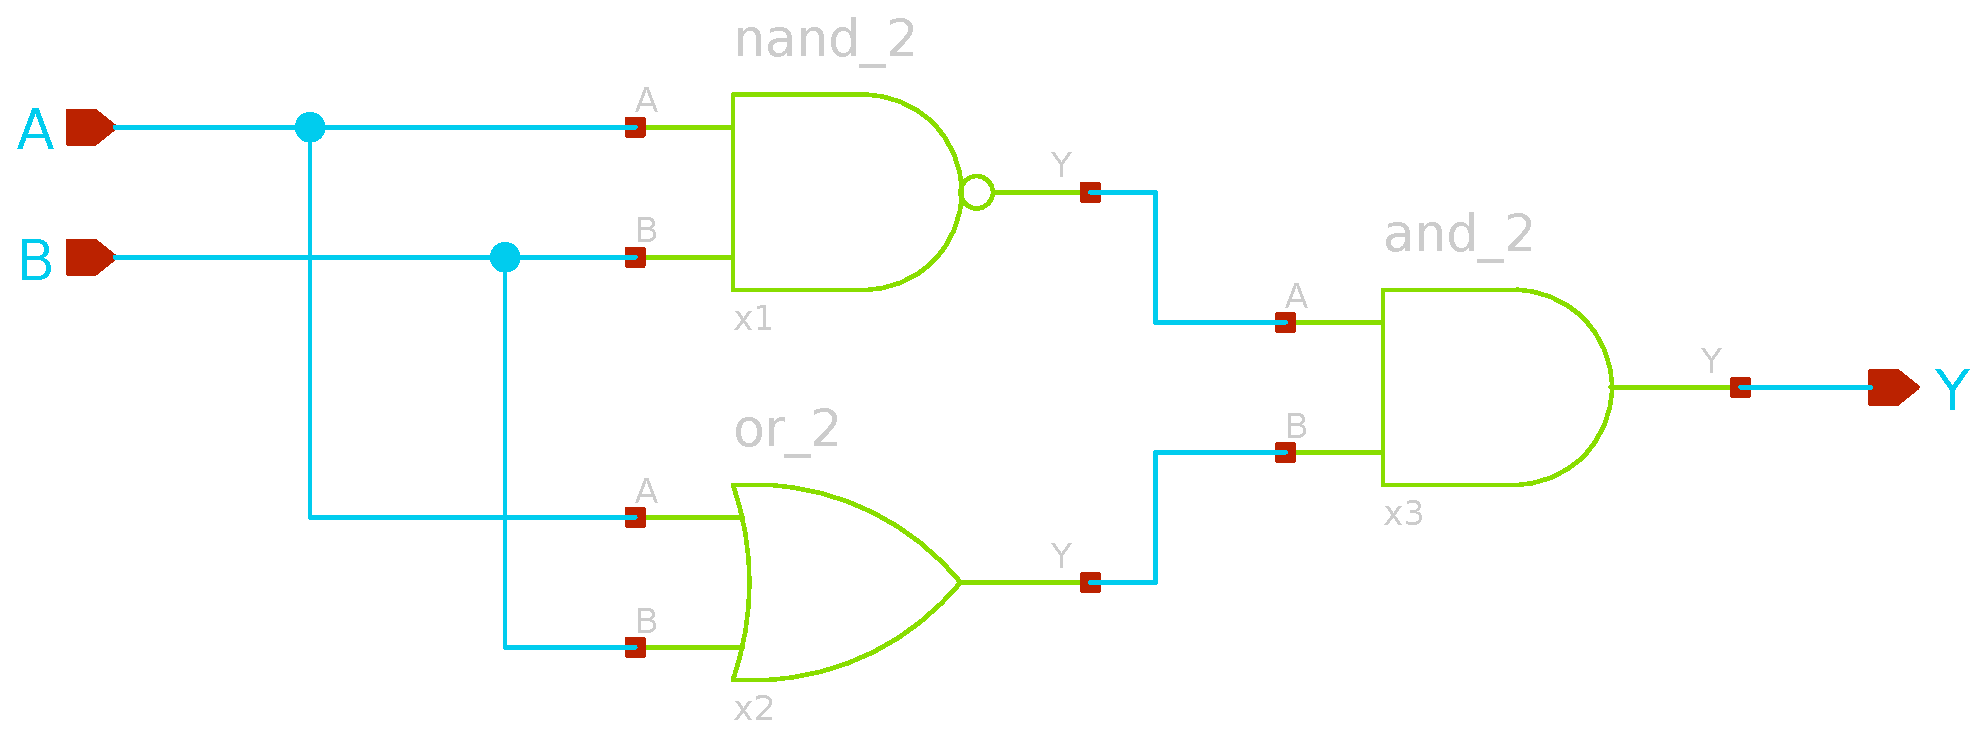
\includegraphics[width=8cm]{Immagini/xor-gate}
			\caption{}
		\end{subfigure}
		\caption{schema rappresentativo del gate xor (a) e relativa costruzione mediante l'utilizzo di altre porte logiche (b).}
		\label{fig:xor}
	\end{figure}

\section{Prestazione dei gate logici}
	Avendo implementato in tecnologia c-mos i vari gate logici e avendone valutato le prestazioni, è possibile iniziare a teorizzare le velocità dei circuiti logici che essi potranno costituire.
	
	Considerando la capacità di carico di $0.75pF$ per tutti i circuiti utilizzati, si osserva che il transitorio di carica/scarica maggiore è associato alla porta logica and con un periodo $\tau$ pari a $7.31ns$: questo permette dunque di stabilire la massima frequenza $f$ cui possono operare i circuiti senza perdere la corretta funzionalità del circuito:
	\[ f = \frac 1 \tau \approx 136 MHz\]
	
	Questo valore di riferimento tuttavia non può essere identificativo della velocità cui può funzionare un circuito logico più complesso, in quanto l'interconnessione di più porte logiche può aumentare la capacità equivalente di carico e dunque il tempo di propagazione del segnale all'interno del circuito.
	
	Per migliorare la stabilità nel funzionamento è possibile supporre che all'interno di un ciclo di clock il tempo legato al transitorio sia il $10\%$ del periodo complessivo: questo dunque riduce la frequenza di operatività del circuito al valore
	\[ f \approx 13.6 MHz \]
	
	Questo valore di sicurezza permette così di stabilire una frequenza di operatività del circuito che assicuri una corretta trasmissione dei dati all'interno delle varie sezioni circuitali che compongono un microprocessore.
	
	
	























\textbf{MAGARI FARE DELLE CONSIDERAZIONI SULLE PRESTAZIONI, COME LA MASSIMA FREQUENZA DI COMMUTAZIONE?}